\section{Tool calls}
\label{sec:toolcalls}

Lecture~3 drew the tools node of \msa{} as a single box (\cref{sec:recap}), and this section opens
it. We define a tool call, the harness that executes it and the boundaries that the call crosses, and
we follow the history of tool calling from remote procedure calls to the Model Context Protocol. The
history matters for design, because once a tool runs outside the harness's process, a call can fail
without a reply, and a retry can repeat its effect. The section ends with the terms that describe
such failures and with a design question about which component should prevent a repeated effect.

\subsection{What a tool call is}
\label{sec:toolcalls-what}

A tool call is a request that the model generates and another component executes. Lecture~2
introduced a tool call as a request to run one of the agent's tools, such as \demoref{read\_file},
with arguments. The model writes the request, and it never runs the tool itself.

The component that executes the request is the harness. The \textbf{harness} is the program that
runs the model loop and executes tool calls on the model's behalf. In \msa{}, the harness consists
of the graph that Lecture~3 studied and the dispatcher, the component that executes each tool call
(\cref{sec:dispatcher}). Lectures~2 and~3 called this program the runtime. From this lecture on, we
call it the harness.

Every tool call passes through the following operations, and each check on a call belongs to one of
them:
\be
\item \textbf{Find.} The harness finds the tool by its name. The name \demoref{edit}, for example,
selects the function that edits a file.
\item \textbf{Bind.} The harness binds the arguments to the parameters, matching each argument in
the request to a parameter of the tool's function.
\item \textbf{Check.} The harness checks \textbf{policy}, the rules that decide whether a requested
call is allowed. A rule might say, for example, that the agent may change only the files in its own
copy of the code.
\item \textbf{Run.} The tool runs and carries out the requested operation.
\item \textbf{Observe.} The harness observes the result and returns it to the model as an
observation, the tool's result as the harness records it (Lecture~2).
\ee
The model performs none of these operations. In this general description, the harness performs all
of them except running the tool. In \msa{}, the check that a path lies inside the agent's copy of
the code runs as the first step inside \demoref{read\_file} and \demoref{edit}, before either tool
touches a file. \Cref{sec:dispatcher} shows which component of \msa{} carries out each operation.

What a tool does, and what the harness must check, is written down in the tool's contract. A
\textbf{tool contract} is the written specification of a tool: what it does, which arguments it
accepts, its results and errors, its side effects and its execution constraints. A \textbf{side
effect} is a change that a call makes outside the caller, such as an edit to a file.
\Cref{sec:dispatcher} examines each part of a contract.

A tool call crosses two boundaries. A \textbf{boundary} is an interface that a request and its reply
cross. The first boundary lies between the model and the harness. The request leaves the model as
part of its reply, and the observation returns to the model as part of its next input. The second
boundary lies between the harness and the tool. The tool may be a function in the harness's own
process, or it may run in another process or on another machine.

Where the tool runs determines which guarantees a call has without extra code. When the tool is a
function in the harness's own process, calling it is a local call. A \textbf{local call} is a call
to a procedure in the caller's own process. If a local call returns, the tool ran, and it ran once.
If the tool fails, an exception reports why.

Across a process or machine boundary, the call loses these guarantees. The tool's contract and the
harness must then supply them explicitly. \Cref{sec:native} lists the guarantees of a local call,
and the history of tool calling (\cref{sec:toolcalls-history}) shows how a boundary takes them away.

\subsection{The history of tool calling}
\label{sec:toolcalls-history}

The history of tool calling divides into two periods: a pre-history before 2022 and a history that
begins around 2022. The pre-history concerns ordinary programs that call procedures on other
machines. The history concerns language models that request tools. The stages are the following:
\bi
\item \textbf{Before 2022.} Work on remote procedure calls, published in 1984 and 1994, established
that a remote call can fail in ways that a local call cannot (\cref{sec:toolcalls-rpc}).
\item \textbf{Around 2022.} Models wrote tool actions as text, and the harness parsed them. This
stage runs from WebGPT in December 2021 to ReAct in October 2022, and Toolformer, posted in
February 2023, also wrote its calls as text (\cref{sec:toolcalls-text}).
\item \textbf{2023 and 2024.} The model API began to return each call in a structured field of its
response, and later guaranteed that its arguments match a schema (\cref{sec:toolcalls-schemas}).
\item \textbf{Late 2024.} The Model Context Protocol moved the tool into its own process
(\cref{sec:toolcalls-mcp}).
\item \textbf{By 2026.} Studies measured how tool calls fail in real systems
(\cref{sec:toolcalls-studies}).
\ei

We describe each stage up to the Model Context Protocol by answering the following questions. What
could the caller or the model do? What did the interface promise? What still went wrong?
\Cref{tab:toolcalls-history}, at the end of \cref{sec:toolcalls-mcp}, collects the answers.

Remote procedure calls also introduced the problem that returns at the end of this history. A call
that crosses a boundary may fail without a reply, and its caller then cannot know whether the call
took effect.

\subsection{Remote procedure calls and partial failure}
\label{sec:toolcalls-rpc}

Remote procedure calls brought a way to fail that local calls do not have. A local call
(\cref{sec:toolcalls-what}) runs the procedure in the caller's own process. A \textbf{remote
procedure call} (\textbf{RPC}) is a call to a procedure on another machine, made to look like a
local call. The caller writes an ordinary call. The RPC system sends the arguments to the other
machine in a message, runs the procedure there, and returns its result to the caller in a reply.

The RPC system of 1984 promised \textbf{at-most-once semantics}, the guarantee that the effect of a
call happens zero times or once.

\begin{definition}[The call semantics of a remote procedure call]
\label{def:toolcalls-rpc}
``We guarantee that if the call returns to the user then the procedure in the server has been
invoked precisely once. Otherwise, an exception is reported to the user and the procedure will have
been invoked either once or not at all---the user is not told which.''
\citep[\S3.1]{birrell1984rpc}
\end{definition}

In the quotation, the user is the calling program, and the server is the machine that runs the
procedure. The guarantee has two halves. A call that returns ran the procedure exactly once. A call
that ends in an exception ran it at most once, and the caller does not learn whether it ran.

The same design prevented a resent message from running a procedure a second time. The
\textbf{transport} is the part of the system that carries messages between the machines. It resent
any message that might have been lost. Each call message carried an identifier for the call, and the
callee discarded any message whose identifier it had already seen.

This protection covers only the copies that the transport makes. Suppose the calling program
receives an exception and calls the procedure again. It then makes a new call with a new identifier,
and the callee runs it as a new call. A retry that the calling program issues is therefore a new
request.

What still went wrong was \textbf{partial failure}: one part of a system fails while the other parts
continue to run. Partial failure is one of the ways in which remote calls differ from local calls.
They also differ in latency, in memory access and in concurrency \citep[\S4]{waldo1994note}.

In a local call, the caller and the callee run in one process. A failure there either stops both of
them or reaches the caller as an exception. Across a boundary, the callee can crash, or a message
can be lost, while the caller keeps running. The caller then waits for a reply that never comes.

A lost request, a crashed callee and a lost reply all look the same to the caller: no reply arrives.
With no reply, the caller cannot tell whether the callee ran. \Cref{fig:toolcalls-local-remote}
contrasts the two kinds of call. In its right half, the callee has run, and only the reply is lost.

\begin{figure*}[t]
  \centering
  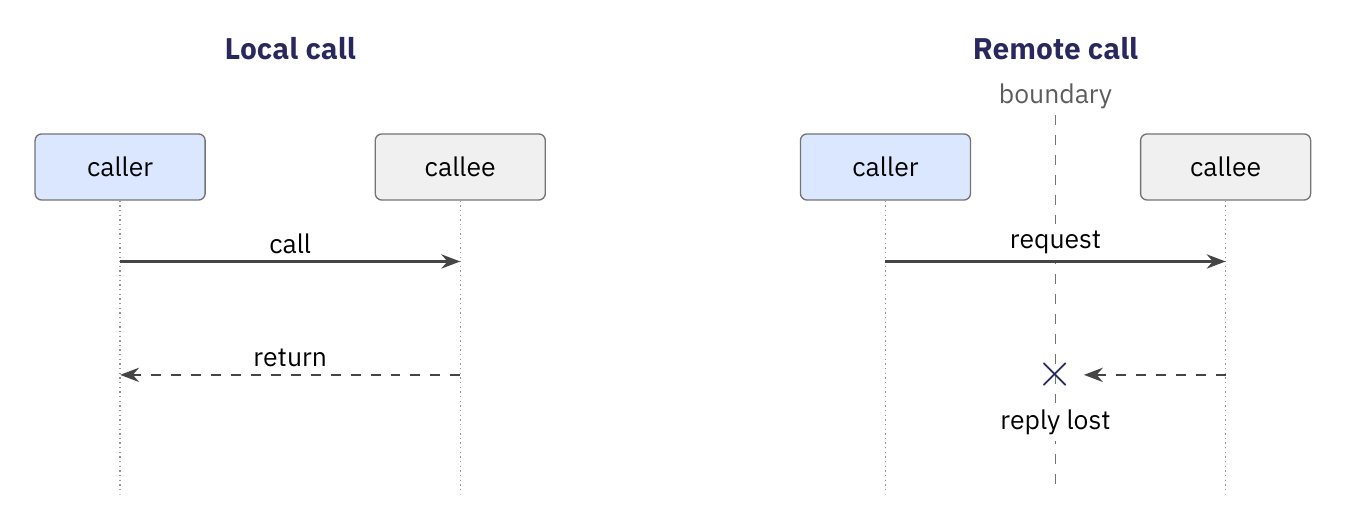
\includegraphics[width=0.7\textwidth]{figures/deck/300b345a5e.png}
  \caption{A local call and a remote call. In the local call, the callee's return reaches the
  caller. In the remote call, the request crosses a boundary and the callee runs, but its reply is
  lost, so the caller cannot tell whether the callee ran.}
  \label{fig:toolcalls-local-remote}
\end{figure*}

\subsection{Tool calls written as text}
\label{sec:toolcalls-text}

The first language models that used tools wrote their actions as ordinary text, and the harness had
to parse that text. WebGPT (December 2021) had the model issue commands to a text-based web browser
\citep{nakano2021webgpt}. MRKL systems (May 2022) routed text to separate tools
\citep{karpas2022mrkl}. ReAct (posted in October 2022 and presented at ICLR 2023) interleaved
reasoning with such actions \citep{yao2023react}. Toolformer, posted a few months later, in February
2023, trained a model to insert calls to APIs into its own text \citep{schick2023toolformer}.

Toolformer's model learned its call format in training. In ReAct, the prompt described the format.
In both systems, the call existed only as text, which the application had to find and parse. We call
the prompt-based form of this approach prompted calling. In \textbf{prompted calling}, the prompt
describes an action format, the model writes the action as text in that format, and the application
that called the model parses it. In our setting, that application is the harness.

\Cref{lst:toolcalls-react} shows an illustrative call in the style of ReAct. The model first writes
a thought, a passage of reasoning (Lecture~2). It then writes an action line, which names the tool
\demoref{edit} and gives its arguments in brackets. The harness finds the action line, splits it
into the tool's name and its arguments, runs the tool, and writes the result after
\texttt{Observation:}.

\begin{lstlisting}[float=tbp, basicstyle=\ttfamily\footnotesize, caption={An illustrative tool call written as text, in the style of ReAct.}, label=lst:toolcalls-react]
Thought: The loop bound in parse() is off by one.
Action: edit[src/parse.py, replace "i <= n" with "i < n"]
Observation: ok
\end{lstlisting}

The interface promised nothing. In prompted calling, the action format lived only in the prompt, and
nothing outside the prompt defined the call. Harnesses of this period typically found the action by
pattern matching. A pattern might, for example, look for a line that begins with \texttt{Action:}
and split the rest of that line at its brackets and commas.

What still went wrong was parsing. A malformed action line, such as one with a missing bracket or a
misspelled tool name, was rejected. An ambiguous action line was misread. Suppose the replacement text
in \cref{lst:toolcalls-react} itself contained a comma. A parser that splits the arguments at commas
would then cut the replacement in two and pass the wrong arguments to the tool. \Cref{sec:native}
returns to this example.

In this stage, the model, the prompt and the parser had to agree on a format that no interface
enforced.

\subsection{Tool schemas in the model API}
\label{sec:toolcalls-schemas}

In 2023 and 2024, the model API itself began to return tool calls in structured fields, and a schema
came to fix the shape of their arguments. OpenAI introduced this change in steps between June 2023
and August 2024.

In June 2023, the API began to return a call as a JSON object, separate from the text of the reply
\citep{openai2023functioncalling}. In \textbf{native tool calling}, the application's request to the
model API lists the available tools, and the response returns each call in its own structured field.
The request describes the arguments of each tool with a JSON Schema, a standard notation for the
names and types of the fields that a JSON object must have. The calling is native because the call
is part of the model API itself. OpenAI calls this function calling, and \cref{sec:native} studies it
in detail.

In November 2023, a single reply could contain several calls \citep{openai2023devday}.
\textbf{Parallel tool calls} are several tool calls in one reply, each with its own identifier. The
identifier lets the harness match each result to the call that it answers. The word parallel means
that the calls arrive together in one reply. The harness may still run them one after another
(\cref{sec:native}).

In August 2024, OpenAI added strict mode \citep{openai2024structuredoutputs}. \textbf{Strict mode} is
an option, set on each tool that the request lists, that guarantees that the arguments of each call
match the schema, within the subset of JSON Schema that strict mode supports. Before strict mode,
nothing in the API enforced the schema, and whether a call matched it was only a tendency of the
model. With strict mode, matching became a guarantee.

The vendor reports that, on its own evaluation of complex schema following, its new model of August
2024 with strict mode scored 100 percent, while an older model that relied on prompting alone scored
under 40 percent. This headline comparison changes the model and the method at once. The same post
also scores the new model with prompting alone and with strict mode off. Those results, rather than
the headline, show what strict mode adds on one model.

\Cref{lst:toolcalls-openai} shows an abbreviated call in OpenAI's chat format
\citep{openai-function-calling}. The call carries the identifier \texttt{call\_7}, the type
\texttt{function} and the name of the tool. Its arguments arrive as a string that contains JSON.
The application must parse that string before it can bind the arguments.

\begin{lstlisting}[basicstyle=\ttfamily\footnotesize, caption={An illustrative tool call in OpenAI's chat format, abbreviated. The arguments arrive as a string.}, label=lst:toolcalls-openai]
{ "id": "call_7",
  "type": "function",
  "function": {
    "name": "edit",
    "arguments": "{\"path\": \"src/parse.py\", ...}" } }
\end{lstlisting}

What still went wrong concerned the values of the arguments: a call can match its schema and still
name the wrong file. Suppose the off-by-one error lies in another file, and the model asks to edit
\texttt{src/parse.py}. The path is a string, as the schema requires, so the call is valid. The schema
guarantee covers the shape of the arguments: their names, their types and the fields that must be
present. It does not cover whether their values are right or what the call will do.

Both guarantees, that a call arrives in a structured field and that its arguments match the schema,
describe only the message that the API returns. The harness must still find the tool, bind the
arguments and check policy before the tool runs, and nothing in the API controls those steps.

\subsection{Tools in another process}
\label{sec:toolcalls-mcp}

In late 2024, the Model Context Protocol moved tools out of the harness's process. The
\textbf{Model Context Protocol} (\textbf{MCP}) is an open protocol that standardizes how a client
lists and calls the tools that a server offers in another process. Anthropic introduced it in
November 2024 \citep{anthropic2024mcp}. The \textbf{client} is the part of the harness that
exchanges messages with a server, and the \textbf{server} is a separate program that offers tools
and runs them. Lecture~5 studies MCP itself.

With MCP, the model could use any tool that a server listed. Every server describes its tools in the
same way, so a harness that implements MCP can use tools that were written without that harness in
mind.

The interface promised one standard for discovery, for the schemas of tool arguments, for results
and for errors. Discovery is the step in which the client asks a server which tools it offers.

In its current revision, the specification defines stdio and Streamable HTTP as its standard
transports, the ways in which
messages travel between the client and the server \citep{mcp-spec-2026-07-28}. Over stdio, the
server runs as a subprocess of the client, and messages travel over its standard input and output.
Over Streamable HTTP, the client sends each message to the server as an HTTP POST request. The reply
returns in the HTTP response, either as a single JSON object or as a stream of events.

MCP encodes every message in JSON-RPC, a standard format for remote calls written in JSON. A
JSON-RPC request names a method and carries an identifier that its reply repeats.
\Cref{lst:toolcalls-mcp} shows an abbreviated request. Its method, \texttt{tools/call}, asks the
server to call a tool. Its parameters name the tool, \demoref{edit}, and give the arguments. Its
id, 7, identifies the request, so that the client can match the reply to it. The request is
illustrative. The tools of \msa{} run in the harness's own process.

\begin{lstlisting}[basicstyle=\ttfamily\footnotesize, caption={An illustrative MCP request that calls the tool \texttt{edit}, abbreviated.}, label=lst:toolcalls-mcp]
{ "jsonrpc": "2.0",
  "id": 7,
  "method": "tools/call",
  "params": { "name": "edit", "arguments": { ... } } }
\end{lstlisting}

What still went wrong was the old problem of the RPC era. A call became a message, and a message can
be lost, delayed, or sent again by a retry. The harness can send this request and never learn
whether the server acted on it. This is the partial failure of \cref{sec:toolcalls-rpc}. It returns
as soon as the tool leaves the harness's process.

\Cref{tab:toolcalls-history} summarizes the stages of the history with the questions of
\cref{sec:toolcalls-history}. Its last column shows how the main failure changed from one stage to
the next. Text actions failed at parsing. Calls returned under a schema could still carry wrong
values, because the schema covers only their shape. Moving tools into separate processes brought
back the partial failure of remote procedure calls.

\begin{table*}[t]
  \caption{The stages of the history of tool calling: what the caller or the model could do, what
  the interface promised, and what still went wrong.}
  \label{tab:toolcalls-history}
  \begin{adjustbox}{width=\linewidth}\begin{tabularx}{\linewidth}{L{0.19\linewidth}XXX}
    \toprule
    \textbf{Stage} & \textbf{What the caller or the model could do} & \textbf{What the interface
    promised} & \textbf{What still went wrong} \\
    \midrule
    \textbf{Remote procedure calls (1984 and 1994)} & A program could call a procedure on another
    machine as if the call were local. & At-most-once semantics: a call that returns ran the
    procedure once, and an exception means once or not at all. & Partial failure: when no reply
    arrives, the caller cannot tell whether the callee ran. \\ \addlinespace
    \textbf{Text actions (2021 to early 2023)} & The model could write an action as text, which the
    harness parsed. & Nothing: the action format lived only in the prompt. & Parsing: a malformed or
    ambiguous action line was rejected or misread. \\ \addlinespace
    \textbf{Schemas in the model API (2023 and 2024)} & The model could return a call as JSON, and
    several calls in one reply, each with an identifier. & Each call arrives in its own structured
    field (2023). With strict mode (2024), its arguments match the schema. & Wrong values: a call can match the schema
    and still name the wrong file. \\ \addlinespace
    \textbf{Tools in another process (MCP, from 2024)} & The model could use any tool that a server
    listed. & One standard for discovery, schemas of tool arguments, results and errors, over stdio
    and, in the current revision, Streamable HTTP. & The problem of the RPC era: a message can be lost, delayed, or sent again
    by a retry. \\
    \bottomrule
  \end{tabularx}\end{adjustbox}
\end{table*}

\subsection{Studies of tool-call failures}
\label{sec:toolcalls-studies}

By 2026, studies had begun to measure how tool calls fail in real systems. They include fault
catalogs, injected-fault benchmarks and a study of checkpoint-restore:
\bi
\item \textbf{Fault catalogs.} A fault catalog classifies the failures found in real software. Two
studies of 2026 grouped real failures of MCP software into named categories
\citep{taraghi2026mcpfaults,owotogbe2026mcpruntime}.
\item \textbf{Injected-fault benchmarks.} A benchmark of this kind makes tools fail on purpose
during a run, for example by letting them time out, limit the rate of requests or return partial
results. A benchmark of January 2026 measured how far the success of agents falls under such faults
\citep{gupta2026reliabilitybench}.
\item \textbf{A study of checkpoint-restore.} A checkpoint saves a run's progress so that the run can
resume from that point (Lecture~2). Agent frameworks that offer checkpoint-restore advise developers
to make tool calls safe to retry. A study of March 2026 examined whether this advice prevents
duplicate effects at the tool boundary \citep{zheng2026acrfence}. After a restore, the agent
regenerates its requests, and they differ slightly from the original ones. Servers treat them as new
requests, so irreversible effects, such as a payment, can happen again.
\ei
Together, these studies treat failures at the tool boundary, including timeouts and repeated
effects, as events that can be observed, classified and measured.

\subsection{A retried request}
\label{sec:toolcalls-retry}

A retried request can apply the same patch twice. Consider a harness that calls a tool on an MCP
server, and suppose that the tool applies a patch to a file. \Cref{fig:toolcalls-retry} draws the
exchange with time running downward. On the server's side, it shows the patch applied once for the
request with id 7 and again for the request with id 8. The scenario unfolds as follows:
\bi
\item \textbf{The request.} The request with id 7 reaches the server, and the server applies the
patch.
\item \textbf{The reply.} The reply never reaches the harness. After waiting for a set time, the
harness gives up, and the request has timed out. The harness cannot tell whether the patch was
applied.
\item \textbf{The retry.} The harness sends the request again. The retry is a new request with id 8,
and the server applies the patch a second time.
\ei

\begin{figure*}[t]
  \centering
  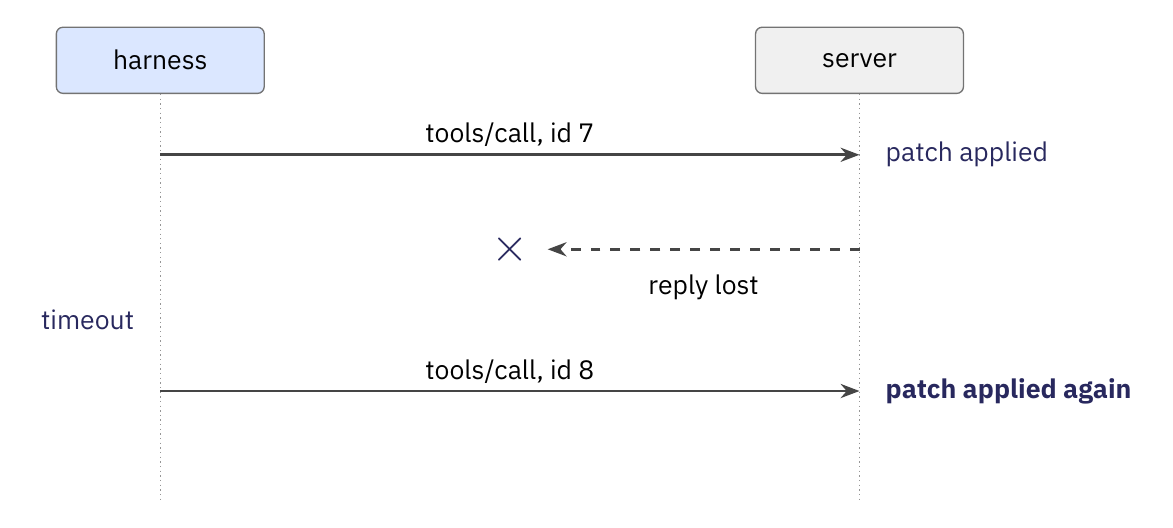
\includegraphics[width=0.6\textwidth]{figures/deck/a9a99892bc.png}
  \caption{A retried request applies the same patch twice. The server applies the patch for the
  request with id 7, but its reply is lost. The harness times out and sends the request again with
  id 8, and the server applies the patch again.}
  \label{fig:toolcalls-retry}
\end{figure*}

Nothing in MCP lets the server recognize the retry. The relevant rules of MCP, in its revision
2026-07-28, are the following \citep{mcp-spec-2026-07-28}:
\bi
\item \textbf{A broken stream cannot be resumed.} Over Streamable HTTP, a reply that the server
streams travels on a response stream, the open HTTP response that carries the server's messages for
that one request. A stream that breaks cannot be resumed, so a reply lost with it cannot be fetched
again.
\item \textbf{Closing the stream cancels the request.} Over Streamable HTTP, the server must treat
the client's closing of the response stream as a cancellation of the request. The server may
already have finished the work when the cancellation arrives.
\item \textbf{The id matches replies to requests.} A request's id must differ from the id of every
request that is still awaiting its reply. The id tells the client which reply answers which request.
It does not tell the server that a request repeats an earlier one.
\item \textbf{No field marks a repeat.} The core protocol has no field that marks a request as a
repeat of another.
\ei
A retry is therefore a separate request with its own id. The server cannot tell it from a first
request, so it runs the tool again.

From the harness's side, both choices after a missing reply carry a risk. With no reply, the harness
cannot tell a lost request from a lost reply. If it does not retry and the request was lost, the
patch is never applied. If it retries and the reply was lost, the patch is applied twice.

\subsection{Terms for calls across a boundary}
\label{sec:toolcalls-terms}

The scenario of \cref{sec:toolcalls-retry} can be stated precisely with the terms below. They build
on two terms of \cref{sec:toolcalls-what}: the harness, which runs the model loop and executes tool
calls, and a boundary, an interface that a request and its reply cross. Across a process or machine
boundary, a function call becomes a message that can be lost, delayed or delivered twice.

The semantics of a call states how many times its side effect occurs. Under at-most-once semantics
(\cref{sec:toolcalls-rpc}), the effect occurs zero times or once. Under \textbf{at-least-once
semantics}, it occurs one or more times. Under \textbf{exactly-once semantics}, a side effect occurs
once despite lost requests, lost replies or duplicate delivery. \Cref{tab:toolcalls-semantics}
compares these semantics, and its last column gives the risk under each when no reply arrives.

\begin{table}[htbp]
  \caption{Semantics of a call that crosses a boundary: how often the effect occurs, and the risk
  when no reply arrives.}
  \label{tab:toolcalls-semantics}
  \begin{adjustbox}{width=\linewidth}\begin{tabularx}{\linewidth}{L{0.25\linewidth}L{0.24\linewidth}X}
    \toprule
    \textbf{Semantics} & \textbf{The effect occurs} & \textbf{Risk when no reply arrives} \\
    \midrule
    \textbf{At-most-once} & Zero times or once & A missing effect, when the caller does not retry
    and the request was lost \\ \addlinespace
    \textbf{At-least-once} & One or more times & A repeated effect, when the caller retries and only
    the reply was lost \\ \addlinespace
    \textbf{Exactly-once} & Once & Neither a missing nor a repeated effect, provided that a repeated
    request has no further effect \\
    \bottomrule
  \end{tabularx}\end{adjustbox}
\end{table}

A harness that never retries obtains at-most-once semantics. A harness that retries until it
receives a reply obtains at-least-once semantics, and the scenario of \cref{sec:toolcalls-retry}
shows the cost: the patch was applied twice. Exactly-once semantics needs both a retry and a
receiver for which a repeated request has no further effect.

A repeated request has no further effect in two cases. In the first, the request is idempotent. An
\textbf{idempotent request} has the same effect when repeated as when executed once. In \msa{},
requests to \demoref{read\_file} and \demoref{search} are idempotent, because these tools only read
files, so repeating them changes nothing. The patch request of the scenario is not idempotent,
because each execution applies the patch again.

In the second case, the receiver recognizes the repeat. An \textbf{idempotency key} is an identifier
that a request carries so that the receiver can detect a duplicate and avoid repeating its effect.
The original request and every retry of it carry the same key. A receiver that remembers the keys it
has processed can then decline a request whose key it has already seen.

The request id of \cref{lst:toolcalls-mcp} cannot serve as an idempotency key, because a retry
carries a new id. The identifier that the RPC system of 1984 attached to each call served this
purpose, but only for the copies that its transport made (\cref{sec:toolcalls-rpc}).

\subsection{Which component should prevent a repeated patch}
\label{sec:toolcalls-question}

The scenario raises a design question. The harness sends a request that applies a patch and
receives no reply. Which component is responsible for ensuring that the patch is applied once?

The duty could fall to the model, which can check the state of the file before it asks for the
patch again. It could fall to the harness, which decides whether to retry. It could fall to the tool
contract, which can accept a key that marks a repeat. In the scenario as described, no component
holds it.

Any answer must respect the following facts:
\bi
\item \textbf{A missing reply is ambiguous.} The absence of a reply does not distinguish a lost
request from a lost reply (\cref{sec:toolcalls-retry}).
\item \textbf{Retries create duplicates.} Any component that retries must therefore allow for
duplicate requests.
\item \textbf{A key lets the receiver decline.} An idempotency key in the tool's contract is the
mechanism that lets the receiver recognize a duplicate and decline it
(\cref{sec:toolcalls-terms}).
\ei

The question is an instance of a broader one: which component enforces a given guarantee?
\Cref{sec:dispatcher} asks it for each guarantee that the harness of \msa{} provides.

\subsection*{Key points}
\bi
\item A tool call is a request that the model generates and the harness executes: the harness finds
the tool by name, binds the arguments and checks policy, the tool runs, and the harness returns the
observed result to the model.
\item A tool call crosses two boundaries, model to harness and harness to tool, and once the tool
runs outside the harness's process, the contract and the harness must supply the guarantees of a
local call explicitly.
\item Remote procedure calls promised at-most-once semantics, but under partial failure a caller
that receives no reply cannot tell whether the callee ran.
\item Prompted calling defined the call only in the prompt, so the harness had to parse actions from
text and could reject or misread them.
\item Native tool calling returns each call in a structured field, and strict mode guarantees only
the shape of its arguments, so the harness must still find, bind and check the call before the tool
runs.
\item MCP moved tools into separate server processes, so a call became a message that can be lost,
and a retry carries a new id that the server cannot recognize as a repeat.
\item Any component that retries must allow for duplicate requests, and exactly-once semantics needs
a repeated request to have no further effect, either because the request is idempotent or because an
idempotency key lets the receiver decline it.
\ei
